  % --------------------------------------
% Document Class
% --------------------------------------
\documentclass[a4paper,11pt]{article}
% --------------------------------------



% --------------------------------------
% Use Package
% --------------------------------------


\usepackage[francais]{babel}
%\usepackage{ucs}
\usepackage[utf8]{inputenc}
\usepackage[T1]{fontenc}

\usepackage{makeidx}
\usepackage{color}
\usepackage{graphicx}
\usepackage{float}
\usepackage[hidelinks]{hyperref} 
\usepackage{geometry}
%\usepackage{lastpage}
%\usepackage{marginnote}
\usepackage{fancyhdr}
%\usepackage{titlesec}
%\usepackage{framed}
\usepackage{amsmath}
\usepackage{empheq}
\usepackage{array}
\usepackage{multicol}
\usepackage{csquotes}
%\usepackage{adjustbox}

% insert code
\usepackage{listings}

% define our color
\usepackage{xcolor}

% code color
\definecolor{ligthyellow}{RGB}{250,247,220}
\definecolor{darkblue}{RGB}{5,10,85}
\definecolor{ligthblue}{RGB}{1,147,128}
\definecolor{darkgreen}{RGB}{8,120,51}
\definecolor{darkred}{RGB}{160,0,0}

% other color
\definecolor{ivi}{RGB}{141,107,185}


\lstset{
  language=R,
  captionpos=b,
  extendedchars=true,
  frame=lines,
  numbers=left,
  numberstyle=\tiny,
  numbersep=5pt,
  keepspaces=true,
  breaklines=true,
  showspaces=false,
  showstringspaces=false,
  breakatwhitespace=false,
  stepnumber=1,
  showtabs=false,
  tabsize=3,
  basicstyle=\small\ttfamily,
  backgroundcolor=\color{ligthyellow},
  keywordstyle=\color{ligthblue},
  morekeywords={include, printf, uchar},
  identifierstyle=\color{darkblue},
  commentstyle=\color{darkgreen},
  stringstyle=\color{darkred},
}


% --------------------------------------



% --------------------------------------
% Page setting
% --------------------------------------
%\pagestyle{empty}
\setlength{\headheight}{15pt}

\setcounter{secnumdepth}{3}
\setcounter{tocdepth}{2}

\makeatletter
\@addtoreset{chapter}{part}
\makeatother 

\hypersetup{         % parametrage des hyperliens
  colorlinks=true,      % colorise les liens
  breaklinks=true,      % permet les retours à la ligne pour les liens trop longs
  urlcolor= blue,       % couleur des hyperliens
  linkcolor= black,     % couleur des liens internes aux documents (index, figures, tableaux, equations,...)
  citecolor= green      % couleur des liens vers les references bibliographiques
}

% --------------------------------------

% --------------------------------------
% Information
% --------------------------------------
\title{Compte-rendu TP10 RdF\\ \ \\\textbf{Arbres de décision et reconnaissance de visages}\\ \ \\}
\author{Elliot VANEGUE et Gaëtan DEFLANDRE}
% --------------------------------------

\definecolor{myColor}{rgb}{0.5, 0.1, 0.75}

% --------------------------------------
% Begin content
% --------------------------------------
\begin{document}
  
  % Set language to english
  \selectlanguage{francais}
  
  % Start the page counting
  \pagenumbering{arabic}
  
  \maketitle
  
  \mbox{}
  \newpage
  \clearpage
  
  \section{Introduction}
  Dans le cadre de ce TP, nous avons cherché à reconnaître des chiffres grâce à l'utilisation d'arbre
  de décision et de l'entropie pour construire cette arbre. La différence avec le TP que nous avons eu précédemment est que nous avons 
  plusieurs image du même chiffre, ce qui implique une gestion de classe. Chaque classe étant
  un chiffre. Nous allons devoir contruire un arbre sur la base d'image d'apprentissage et tester
  cet arbre avec des images de test afin de voir si cet algorithme reconnaît facilement les chiffres.\\
  
  \section{Préparation des données}
  Pour ce TP, nous travaillons avec une base de chiffre stocké dans plusieurs images. 
  Chaque image correspond à un chiffre et contient 1100 fois ce chiffre. Avant tout, 
  nous binarisons ces images afin d'obtenir des images composées uniquement de 0 et de 1.\\
  
  \begin{figure}[H]
    \centering
    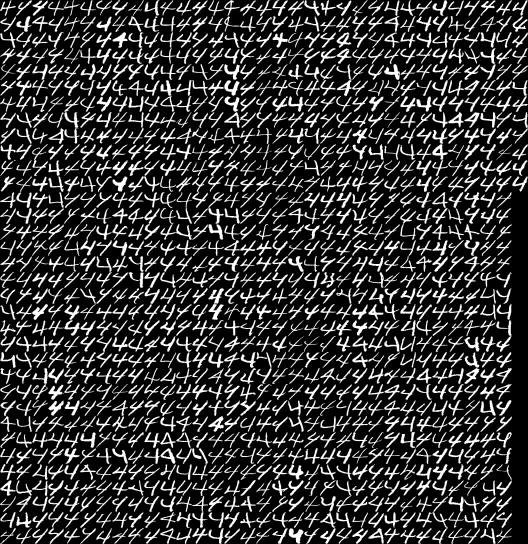
\includegraphics[width=7cm]{usps_4.jpg}
    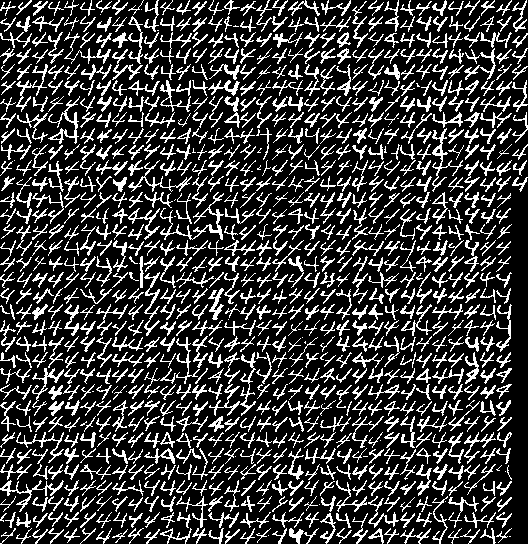
\includegraphics[width=7cm]{usps_4.png}
    \caption{Les données pour l'image des quatres. À gauche, image avant binarisation. À droite, image après binarisation.}
  \end{figure}
  
  Dans un premier temps, nous décomposons chaque image en un tableau à trois dimensions 
  représentant un chiffre avec ces différents exemplaires et leurs pixels. Ensuite, nous
  rassemblons toutes les images (images des classes 528*544) dans un seul même tableau à trois dimensions.
  Les labels des classes de chaque image (image d'un chiffre 16*16) sont aussi calculés.\\
  
  Pour faire ces opérations, nous utilisons les fonctions suivante, écrite par le professeur : 
  
  \begin{lstlisting}[caption=Fonction de décomposition de la base]
splitImageArray <- function( images, rows, cols, height, width ) {
    result <- array( , dim = c( height, width, rows * cols ) );
    for ( i in 1:rows ) {
        for ( j in 1:cols ) {
            result[ , , (j-1)*rows+i ] <- images[((i-1)*height+1):(i*height), ((j-1)*width+1):(j*width)];
        }
    }
    return (result);
}
  \end{lstlisting}
  
  \begin{lstlisting}[caption=Fonction qui lit toutes les images et construit la base et les labels]
readUSPSdata <- function( folder ) {

    # output data: image matrix and labels vectors
    data <- array(, dim=c(16, 16, 0) );
    labels <- vector( , length=0 );

    # read the image files 
    for ( i in 0:9 ) {
        file <- sprintf( "%s/usps_%d.png", folder, i );
        image <- rdfReadGreyImage( file );
        image <- t( imageData( image ) );
        images <- splitImageArray( image, 34, 33, 16, 16 );
        images <- images[ , , 1:1100 ];
        data <- abind( data, images, along=3 );
        labels <- c( labels, rep ( i, 1100 ) );
    } 

    return ( list(data, labels) );
}
  \end{lstlisting}

  
  Caractéristique du tableau à trois dimensions dans l'exemple des chiffres :
  \begin{itemize}
   \item première et deuxième dimension : taille d'une image (16x16).
   \item troisième dimension : nombre total d'image (11000).
  \end{itemize}
  \ \\

  Caractéristique des labels :
  \begin{itemize}
   \item vecteur de numérique de taille le nombre total de'image (11000).
   \item chaque élément du vecteur correspond à la classe de l'image de chiffre (16*16) correspondante.
  \end{itemize}
  
  \section{Méthodologie}
  Afin de pouvoir calculer l'entropie, nous avons besoin dans un premier temps de calculer la probabilité qu'un 
  pixel soit présent dans une classe. Pour cela nous fesons l'addition de toutes les images d'apprentissage d'une classe 
  suivit d'une division par le nombre d'images d'apprentissage pour une classe. Nous choisissons de prendre la moitié
  des images en apprentissage, soit 550 par classes, représenter par le paramètre \enquote{napp}.\\
  
  \begin{lstlisting}[caption=Fonction de calcul de la probabilité de la présence d'un pixel]
probabilityPixelOfClassInNApp <- function( data3D, labels, nnumber, napp, mask ) {

    # width
    W <- 16
    # heigth
    H <- 16

    pc <- array(, dim=c(W, H, 0) );

    # pour chaque classe
    for ( c in 0:9 ) {
        csum <- matrix(rep(0, W*H), nrow=H,ncol=W, byrow=TRUE)
        cpt <- 0

        # pour chaque image de la classe, dans les images d'apprentissage
        # et appartenant aux images du mask 
        for ( i in 1:napp ){
            imgID <- (c * nnumber) + i
            if (mask[imgID]){
                csum <- csum + data3D[,,imgID]
                cpt <- cpt + 1
            }
        }

        csum <- csum / cpt
        pc <- abind( pc, csum, along=3 )
    }

    return ( pc )
}
  \end{lstlisting}
  
  Le paramètre \enquote{mask} est un tableau, de la même compositions que \enquote{data} mais avec des booléens,
  qui permet de déterminer si l'image traité dans la boucle doit être 
  prix en compte pour le calcul ou non. Cela permet de différencier les images d'apprentissage des images de test 
  et par la suite de disqualifier certaines images lors de la descente dans l'arbre et en fonction de l'image testée.
  Cette probabilité va nous permettre de calculer l'entropie comme nous l'avons fait dans le TP précédent mais sur chacune
  des classes et non pas sur chacun des éléments (exemplaire de chiffre).\\
  
  \begin{lstlisting}[caption=Fonction de calcul de l'entropie]
computeEntropy <- function( pc ) {
 
    # width
    W <- 16
    # heigth
    H <- 16

    sum <- matrix(rep(0, W*H), nrow=H,ncol=W, byrow=TRUE)

    for ( c in 0:9 ){
        sum <- sum + ( log2(pc[,,c+1]^pc[,,c+1]) )
    }

    return ( - sum )
}
  \end{lstlisting}
  
  \section{Sélection de pixel}
  Pour sélectionner le pixel qui sera le noeud permettant de partager au mieux l'ensemble en deux, nous prenons
  l'entropie la plus élevé. Nous pouvons alors chercher dans quel ensemble l'image se trouve en regardant si
  elle possède le pixel sélectionné ou non. Ainsi nous éliminons toutes les images qui n'ont pas le même pixel
  que l'image testée. Nous effectuons ce calcule jusqu'une certaines profondeur qui nous premet encore de 
  faire le calcul de l'entropie et nous donne des résultat cohérent.\\
  
  \begin{lstlisting}[caption=Algorithme principal du TP]
findClassFromImgtest <- function( imgtest, data, labels, nnumber, napp, mask ) {

    curentMask <- mask

    repeat {

        pc <- probabilityPixelOfClassInNApp(data, labels, nnumber, napp, curentMask)

        entropy <- computeEntropy(pc)

        # condition d'arret
        if ( is.nan(sum(entropy)) || sum(curentMask)<250 ){
            # on s'arrete: 
            # si il y a des nan dans la matrice entropy
            # ou 
            # si on a déja fait beaucoup d'itération
            break
        }

        bestPixel <- which.max(entropy)

        best.row <- bestPixel %% 16 
        if( best.row==0 ){
            best.row <- 16
        }

        # on arroundit au supérieur car les indices commence à 1
        best.col <- ceiling( bestPixel/16 )

        imagesWithBest <- whichImgContain(best.row, best.col, data, nnumber)

        if(imgtest[best.row,best.col] == 1) {
            curentMask <- imagesWithBest & curentMask
        } else {
            curentMask <- !imagesWithBest & curentMask
        }

    }

    proba <- getProbaComeFromClass(curentMask, napp)

    # on fait -1 car le chiffre 0 commence a l'indice 1
    return  ( which.max(proba) - 1 )
}
  \end{lstlisting}
  
  \newpage
  
  \section{Taux de bonne classification}
  Il est ensuite possible de tester toutes les images de test pour calculer le taux de bonne 
  classification, la classification est correcte si la classe trouvée par l'algorithme est 
  identique aux labels pour l'image testée.

  \begin{lstlisting}[caption=Taux de bonne classification]
# -----------------------------------------------
# TAUX DE BONNE CLASSIFICATION
# (tests sur toutes les images de test)
# -----------------------------------------------

vecBC <- rep(FALSE, ntest*10)

for (c in 0:9){
    print(paste("Test sur la classe", c))
    for (i in 1:(ntest)){
        idData <- (c*nnumber) + napp + i
        idVecBC <- (c*ntest) + i
        foundClass <- findClassFromImgtest( data[,,idData], data, labels, nnumber, napp, nappMask )
        if(foundClass == labels[idData]){
            vecBC[idVecBC] = TRUE
        }
    }
}

tauxBC <- sum(vecBC) / length(vecBC)

print(paste("Taux de bonne clasification", tauxBC))
  \end{lstlisting}
  
  Avec un nombre d'images d'apprentissage de 550 pour chaque classe, dans 23.62\% des images de test
  on retrouve la bonne classification. Ce taux est faible, néanmoins, il est plus de deux fois plus élévé 
  que le hasard, le hasard donne $\frac{1}{10}$ une bonne classification, car il y a 10 classes.
  
  \section{Conclusion}
  Nous avons pu voir que cette méthode de reconnaissance de forme ne permet pas d'avoir un résultat
  très fiable. En effet plusieurs chiffres, sont mal reconnu par l'algorithme étudié lors de ce TP.
  La valeur des pixels sur une image en dégradé de gris ne suffit donc pas, il faudrait utiliser 
  d'avantage de paramètre comme la couleur de la peau ou la position de certaines caractèristique du visage
  pour rendre cette algorithme plus fiable.
  
  Cependant, cette algorithme donne une solution avec peu d'itération.
  
  \newpage
  
  \section{Annexe}
  
  \subsection{Code de la macro utilisant les fonction et calculant le taux de bonne classification}
  \begin{lstlisting}[caption=Macro testant les images de test]
# -----------------------------------------------
# Chargement des fonctions externes
# -----------------------------------------------

library ("EBImage")
library( abind );
source ("rdfTools.R")



# -----------------------------------------------
# DATA ET VARIABLES UTILIES
# -----------------------------------------------

# lecture des images binaires
output <- readUSPSdata("usps")

data <- output[[1]]
labels <- output[[2]]

# nombre d'images par classe
nnumber <- 1100

# la moitie des images sont d'apprentissage (550 sur 1100)
napp <- 550
ntest <- nnumber - napp

# largeur et hauteur d'une image d'un chiffre
width <- 16
heigth <- 16



# -----------------------------------------------
# TEST SUR UNE IMAGE DE TEST
# -----------------------------------------------

# >> ------------ >
#
# IMAGE TEST
#
# Tous les 1100 images on passe a une autre classe (autre chiffre),
# Les images de 1 à 550 sont d'apprentissage.
#
# Par exemple de 1 à 550 c'est l'apprentissage des images de 0 et 
# de 4401 à 4950 c'est l'apprentissage des images de 4
#
# -----------------

imgtest <- data[,,851] # 0
#imgtest <- data[,,1902] # 1
#imgtest <- data[,,3008] # 2
#imgtest <- data[,,4120] # 3
#imgtest <- data[,,5207] # 4
#imgtest <- data[,,6487] # 5
#imgtest <- data[,,7409] # 6
#imgtest <- data[,,8888] # 7
#imgtest <- data[,,9609] # 8
#imgtest <- data[,,10996] # 9

# < ------------ <<

# image considere pour le calcul de l'entropie
nappMask <- getNAppMask(nnumber, napp)

foundClass <- findClassFromImgtest( imgtest, data, labels, nnumber, napp, nappMask )

print(paste("L'image testé appartient probablement à la classe", foundClass))



# -----------------------------------------------
# TAUX DE BONNE CLASSIFICATION
# (tests sur toutes les images de test)
# -----------------------------------------------

vecBC <- rep(FALSE, ntest*10)

for (c in 0:9){
    print(paste("Test sur la classe", c))
    for (i in 1:(ntest)){
        idData <- (c*nnumber) + napp + i
        idVecBC <- (c*ntest) + i
        foundClass <- findClassFromImgtest( data[,,idData], data, labels, nnumber, napp, nappMask )
        if(foundClass == labels[idData]){
            vecBC[idVecBC] = TRUE   
        }
    }
}

tauxBC <- sum(vecBC) / length(vecBC)

print(paste("Taux de bonne clasification", tauxBC))
  \end{lstlisting}

  
  \subsection{Code des fonctions fessant les calculs pour ce TP}
  \begin{lstlisting}[caption=Les fonctions faisant les calculs pour ce TP]
# -------------------------------------------------------
# Ce fichier contient les fonctions utiles pour le tp 10.
# -------------------------------------------------------

# Chargement d'une image en niveaux de gris
rdfReadGreyImage <- function (nom) {
    image <- readImage (nom)
    if (length (dim (image)) == 2) {
        image
    } else {
        channel (image, 'red')
    }
}

splitImageArray <- function( images, rows, cols, height, width ) {
	result <- array( , dim = c( height, width, rows * cols ) );
	for ( i in 1:rows ) {
		for ( j in 1:cols ) {
			result[ , , (j-1)*rows+i ] <- images[((i-1)*height+1):(i*height), ((j-1)*width+1):(j*width)];
		}
	}
	return (result);
}

# read USPS digits files
# Files must be stored in a single folder and their names must have the
# following format : usps_digit.jpg, where digit is in [0;9].
# Image data is stored in a 16x16x11000 array.
# Image matrices are non-transposed 16x16 matrices.
# Image labels is a vector of integers
#
# params: folder - the folder where the files are stored
#
# returns: a list containing image data and image labels (in [0;9])
#
readUSPSdata <- function( folder ) {

	# output data: image matrix and labels vectors
	data <- array(, dim=c(16, 16, 0) );
	labels <- vector( , length=0 );

	# read the image files 
	for ( i in 0:9 ) {
		file <- sprintf( "%s/usps_%d.png", folder, i );
		image <- rdfReadGreyImage( file );
		image <- t( imageData( image ) );
		images <- splitImageArray( image, 34, 33, 16, 16 );
		images <- images[ , , 1:1100 ];
		data <- abind( data, images, along=3 );
		labels <- c( labels, rep ( i, 1100 ) );
	}

	return ( list(data, labels) );
}

# Retourne un vecteur de booleen de taille le nombre total d'images.
# Mettant a vrai les images d'apprentissage et à faux les images de test.
getNAppMask <- function(nnumber, napp) {

    vec <- rep(FALSE, nnumber*10)

    # pour chaque classe
    for ( c in 0:9 ) {

        # pour chaque image de la classe, dans le nombre pour l'apprentissage 
        for ( i in 1:napp ){
            imgID <- (c * nnumber) + i
            vec[imgID] <- TRUE
        }
    }
    
    return ( vec )
}

# Retourne la probabilite pour chaque pixel, s'il appartient aux classes, 
# parmi les images du masque `mask`
probabilityPixelOfClassInNApp <- function( data3D, labels, nnumber, napp, mask ) {

    # width
    W <- 16
    # heigth
    H <- 16

    pc <- array(, dim=c(W, H, 0) );

    # pour chaque classe
    for ( c in 0:9 ) {
        csum <- matrix(rep(0, W*H), nrow=H,ncol=W, byrow=TRUE)
        cpt <- 0

        # pour chaque image de la classe, dans les images d'apprentissage
        # et appartenant aux images du mask 
        for ( i in 1:napp ){
            imgID <- (c * nnumber) + i
            if (mask[imgID]){
                csum <- csum + data3D[,,imgID]
                cpt <- cpt + 1
            }
        }

        csum <- csum / cpt
        pc <- abind( pc, csum, along=3 )
    }

    return ( pc )
}

# Retourne l'entropie calculée avec la formule du cours, avec prise 
# en compte des classes.
# L'entropie maximale donne le pixel qui separe les images au mieux.
# Avec ce pixel on peut retrouver une liste d'images ayant ce pixel et 
# une liste ne l'ayant pas. 
computeEntropy <- function( pc ) {
 
    # width
    W <- 16
    # heigth
    H <- 16

    sum <- matrix(rep(0, W*H), nrow=H,ncol=W, byrow=TRUE)

    for ( c in 0:9 ){
        sum <- sum + ( log2(pc[,,c+1]^pc[,,c+1]) )
    }

    return ( - sum )
}

# Retourne un vecteur de booleen de taille, le nombre total d'image.
# vec[i] == TRUE : le pixel de position `row`, `col` est blanc (à 1) pour l'image i
# vec[i] == FALSE: le pixel de position `row`, `col` est noir (à 0) pour l'image i
whichImgContain <- function( row, col, data, nnumber ) {

    vec <- rep(FALSE, nnumber*10)

    # pour chaque images dans data
    for ( i in 1:(nnumber*10) ) {
        if ( data[row,col,i] == 1 ) {
            vec[i] <- TRUE
        }
    }

    return ( vec )
}

# Retourne la probabilité que l'image fait partie de la classe 
# Image dont on parle est celle testé et dont les calculs on produit 
# le masque `mask` avec les fonctions ci-dessus.
getProbaComeFromClass <- function( mask, napp) {
    
    
    vsum <- rep(0,10)

    # pour chaque classe
    for ( c in 0:9 ) {

        # pour chaque image de la classe, dans les images d'apprentissage 
        for ( i in 1:napp ){

            imgID <- (c * nnumber) + i
            if (mask[imgID]){
                vsum[c+1] <- vsum[c+1] + 1 
            }
        }

        vsum[c+1] <- vsum[c+1] / napp
    }

    return ( vsum )

}

# --------------------------------

# Fonction principale qui utile une grande partie des autres fonctions
# Retourne la classe probable de l'image de test `imgtest`
findClassFromImgtest <- function( imgtest, data, labels, nnumber, napp, mask ) {

    curentMask <- mask

    repeat {

        pc <- probabilityPixelOfClassInNApp(data, labels, nnumber, napp, curentMask)

        entropy <- computeEntropy(pc)

        # condition d'arret
        if ( is.nan(sum(entropy)) || sum(curentMask)<250 ){
            # on s'arrete: 
            # si il y a des nan dans la matrice entropy
            # ou 
            # si on a déja fait beaucoup d'itération
            break
        }

        bestPixel <- which.max(entropy)

        best.row <- bestPixel %% 16 
        if( best.row==0 ){
            best.row <- 16
        }

        # on arroundit au supérieur car les indices commence à 1
        best.col <- ceiling( bestPixel/16 )

        imagesWithBest <- whichImgContain(best.row, best.col, data, nnumber)

        if(imgtest[best.row,best.col] == 1) {
            curentMask <- imagesWithBest & curentMask
        } else {
            curentMask <- !imagesWithBest & curentMask
        }

    }

    proba <- getProbaComeFromClass(curentMask, napp)

    # on fait -1 car le chiffre 0 commence a l'indice 1
    return  ( which.max(proba) - 1 )
}
  \end{lstlisting}

  
\end{document}  